%DO NOT MESS AROUND WITH THE CODE ON THIS PAGE UNLESS YOU %REALLY KNOW WHAT YOU ARE DOING
 \chapter{Random variables and random Numbers}
\noindent \textbf{Random variables:}\\
\noindent Random variable is a way to represent a sample space by assigning one or more numerical values to each outcome. If the outcome produces one value, the probability distribution is univariate and if the outcome produces more than one value the probability distribution is multi variate. If the sample space is finite or countable infinite then random variable is a discrete random variable. A continuous random variable takes uncountably infinite many values in an interval of real numbers.

\noindent \textbf{Probability density function:}\\
\noindent It is a statistical expression that defines a probability distribution for a continuous random variable as opposed to a discrete random variable. When the PDF is graphically portrayed, the area under the curve will indicate the interval in which the variable will fall. The total area in this interval of the graph equals the probability of a continuous random variable occurring.
\begin{figure}[H]
\begin{center}
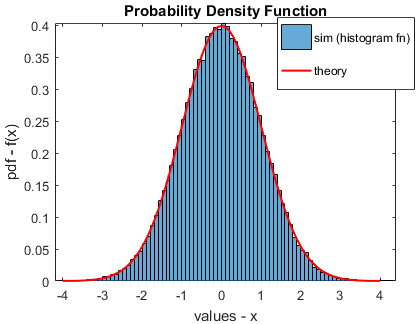
\includegraphics[scale=0.55]{fig12.png}\\
\caption{Probability density function}
\label{Probability density function}
\end{center}
\end{figure}

\section{Uniform distribution}
\noindent \textbf{Task:} Specify the density function, distribution function and determine the expected value and variance of an on the interval \textit{[a, b]} uniformly distributed random variable \textit{X}. 

\noindent \textbf{Solution:}\\
\noindent The uniform distribution is one of the simplest probability distributions. It is a continuous distribution, this means that it takes values within a specified range, e.g. between 0 and 1. And sometimes it is also known as a rectangular distribution. It has a constant probability.\\
\begin{figure}[H]
\begin{center}
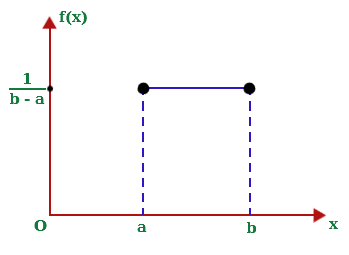
\includegraphics[scale=0.55]{fig10.png}\\
\caption{Uniform distribution of a random variable}
\label{Uniform distribution of a random variable}
\end{center}
\end{figure}
\begin{itemize}
\item Probability density function: It is given by f(x) in the interval [a,b and is defined as,]\\
\[f(x)=
	\begin{cases}
		\text{$\frac{1}{b-a},$} &\quad\text{$a \leq x \leq b$}\\
		\text{0,} &\quad\text{otherwise}
		\end{cases}
\] 

\item Cumulative distribution function: It is method to describe the distribution of random variables. The advantage is that it can be defined for any kind of random variable (discrete, continuous, and mixed). 
The cumulative distribution function (CDF) of random variable $F_X(X)$ is defined as,
 \[F_X(X)=
	\begin{cases}
		\text{0,} &\quad\text{for x$<$a} \\
		\text{$\frac{x-a}{b-a}$,} &\quad\text{for $a \leq x \leq b$}\\		\text{1,} &\quad\text{for x$>$b}
		\end{cases}
\] 
\begin{figure}[H]
\begin{center}
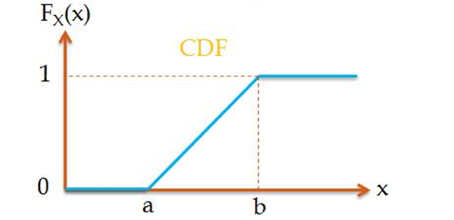
\includegraphics[scale=1.1]{fig11.png}\\
\caption{Cumulative distribution function of a random variable}
\label{Cumulative distribution function of a random variable}
\end{center}
\end{figure}

\item Expected value: It is also called as the mean value. \texttt{E[X]} of the Uniform distributed random variable in the interval [a, b] is given as,\\
\begin{center}E[X]=$\int_{-\infty}^{\infty}Xf(x)dx$\space\space\space\space\space f(x)=$\frac{1}{b-a}$.\end{center}
$$E[X]=\frac{1}{b-a}\int_a^bxdx$$
$$E[X]=\frac{1}{b-a}\left[\frac{x^2}{2}\right]_a^b$$
$$E[X]=\frac{b^2-a^2}{2(b-a)}$$
$$E[X]=\frac{b+a}{2} = \mu $$

\item Variance: \texttt{V[X]} of a Uniformly distributed random variable in the interval [a, b] is as,\\
$$V[X]=\sigma^2=E(X-\mu)^2=E(X^2-2\mu X+\mu^2)$$
$$V[X]=E(X^2)-2E(X)\mu+\mu^2$$
$$V[X]=E(X^2)-(E(X))^2$$
\noindent Therefore by using, $$E[X]=\frac{b+a}{2} = \mu,$$
\noindent we get,
$$V[X] = \frac{(b-a)^2}{12}$$

\end{itemize}
\section{Normal distribution}
\noindent \textbf{Task:} Specify the density function and the distribution function of a ${N(\mu,\sigma^2)}$ distributed random variable \textit{X}. How can the tabulated values of the standard normal distribution function be used to determine values for a ${N(\mu,\sigma^2)}$ distributed random variable?

\noindent \textbf{Solution:}\\
\noindent The normal distribution is an extremely important continuous probability distribution. In probability theory, the normal distribution is also called the Gaussian distribution. There are two parameters in normal distribution, $\mu$ is the mean and lies between $-\infty$ and $+\infty$ and $\sigma$ is the standard deviation.
 
 The normal density function is given by:\\
\begin{center}
$f_x(x)=\frac{1}{\sqrt{2\pi\sigma^2}}\text{exp}\left\{-\frac{(x-\mu)^2}{2\sigma^2}\right\},$ \space\space\space  $X\in R$
\end{center}
The normal distribution function is given by:\\
\begin{center}$F_x(X)=\int\limits_{-\infty}^xf(x')dx'$\\
$F_x(X)=\int_{-\infty}^x\frac{1}{\sqrt{2\pi\sigma^2}}\text{exp}\left\{-\frac{(x-\mu)^2}{2\sigma^2}\right\}dx'$\end{center}
If X is a random variable that has a normal distribution with mean, $\mu$ and variance, $\sigma^2$,we write this equation as $X \sim N$ ($\mu, \sigma^2$). The standard normal distribution with mean 0 and variance 1 and is written as $Y\sim N$ (0,1). Its distribution function is usually denoted by $\phi(x)$.
$$\phi(x)=\frac{1}{\sqrt{2\pi}}\int_{-\infty}^x\text{exp}\left\{-\frac{x'^2}{2}\right\}$$
Let $X \sim N (\mu, \sigma^2)$ and therefore $\frac{(X-\mu)}{\sigma} \sim N(0,1)$ then
$$F_X(x)=P(\{\zeta: -\infty<X(\zeta)\leq x\})$$
$$F_X(x)=P(\{\zeta:-\infty<\frac{X(\zeta)-\mu}{\sigma}\leq \frac{x-\mu}{\sigma}\})=\phi\left\{\frac{x-\mu}{\sigma}\right\}$$
The following graph represents normal distribution curves of various mean and variance values.
\begin{figure}[H]
\begin{center}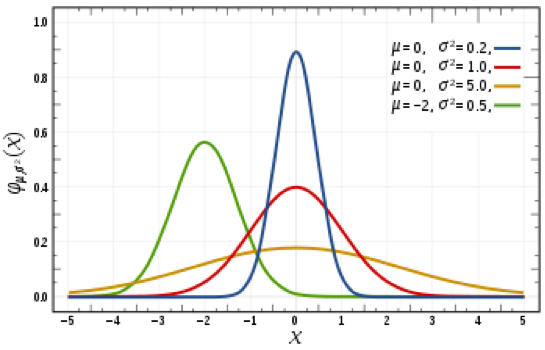
\includegraphics[scale=0.8]{fig13.png}\end{center}
\caption{Normal Distribution Curve}
\label{Normal Distribution Curve}
\end{figure}
 
 
 
\section{Approximation of distribution function}
\noindent \textbf{Task:} What are the advantages in estimating the distribution function instead of estimating the corresponding density function? \\
\noindent \textbf{Solution:} \\
\noindent \textbf{Probability density estimation using histograms:} The histogram partitions the set [0,1] into several bins and uses the count of the bin as a density estimate. The sample space is split up into bins and then the count of the samples that fall into each bin is taken and is divided by the total number of samples. Keeping the width of the bins fixed, as the number of data sampled increases, then by the law of large numbers, the relative frequency for each bin will converge on the bins probability. When the number of bins is too large, the quantity (bias) will be small while the second quantity (variance) will be large. When the number of bins is too small, the quantity (bias) will be large while the second quantity (variance) will be small. This is called over-smoothing. There exists a bias-variance trade off.\\
\noindent \textbf{Probability distribution using histograms:} Suppose we have one-dimensional samples \\\texttt{$x_1:x_2:::x_n$} with a cumulative distribution function \textit{F}. Then we can define the empirical cumulative distribution function on \texttt{n} samples as,
$$ {F_n(x)}^{'} = \frac{1}{n}\sum_{i=1}^{n} 1\{ X_{(i)}\leq x \} $$
\noindent According to Glivenko-Cantelli Lemma, the empirical distribution converges uniformly to \texttt{F(x)}, namely
$$ {max}_{n}|{F_n(x)}^{'} - F(x)| \longrightarrow 0 $$
\noindent The maximum gap between the empirical CDF and true CDF goes. It means we can learn distributions just by collecting enough data.

\section{Bivariate normal distribution}
\noindent \textbf{Task:} Specify the density function $f_{x,y}(x,y)$ and the characteristic function $\varphi_{x,y}(x,y)$ of two bivariate normal distributed random variables \textit{X} and \textit{Y} with the expected values $\mu_x$, $\mu_y$, the variances ${\sigma_x}^2$, ${\sigma_y}^2$  and the correlation coefficient $\rho$. Outline the level curves of the density function\\
 \{\textit{(x,y)}: $f_{x,y}(x,y)$ = const.\} for $\rho = 0$ and $\rho = 1/2.$ To what shape degenerate the level curves in
case of $\rho = \pm 1?$

\noindent \textbf{Solution:} A bivariate distribution is a type of bivariate probability distribution and it represents the generalization of the normal distribution over two dimensions. A two dimensional normal distribution is called as bivariate normal distribution. Two random variables X and Y are said to be bivariate normal, if $aX+bY$ has a normal distribution for all a, b $\in$ R. The density function of a Bivariate Normal Distribution is,\\
$$f_{XY}(x,y)=\frac{1}{2\pi\sigma_x\sigma_y\sqrt{1-\rho^2}}exp\left[-\frac{1}{2(1-\rho^2)}.\{(\frac{x-\mu_x}{\sigma_x})^2-2\rho\frac{(x-\mu_x)(y-\mu_y)}{\sigma_x\sigma_y}+(\frac{y-\mu_y}{\sigma_y})^2\right]$$
For all   $x, y \in R: -1< \rho <1;   \sigma_x >0$ and $\sigma_y >0$\\
\noindent The density function of the Standard Bivariate Normal Distribution can be given as:\\
$$F_{XY}(x,y)=\frac{1}{2\pi\sqrt{1-\rho^2}}\text{exp}\left[-\frac{1}{2(1-\rho^2)}.\{x^2-2\rho xy+y^2\}\right]$$
where, $\sigma \in (-1, 1)$. If $\rho$=0, then we just say X and Y have the standard bivariate normal distribution.
\noindent The characteristic function of the bivariate normal distribution is defined as,
$$\phi_{XY}(t1,t2)=\int_{-\infty}^{\infty}\int_{-\infty}^{\infty} f_{xy}(x,y)exp(j(t1x+t2y)dxdy$$

\noindent If the two random variables X and Y are independent, the characteristic function of the bivariate normal distribution given as,
$$\phi_{XY}(t1,t2)=\text{exp}(j\mu_xt1)\text{exp}\left[\frac{(\sigma_x^2/t1^2)}{2}\right]\text{exp}(j\mu_yt2)\text{exp}\left[\frac{(\sigma_x^2/t2^2)}{2}\right]$$
 \noindent The level curves for the density function are shown in Figure 1.5. 
 
 \begin{figure}[!ht]
   \centering
   \subfloat[][]{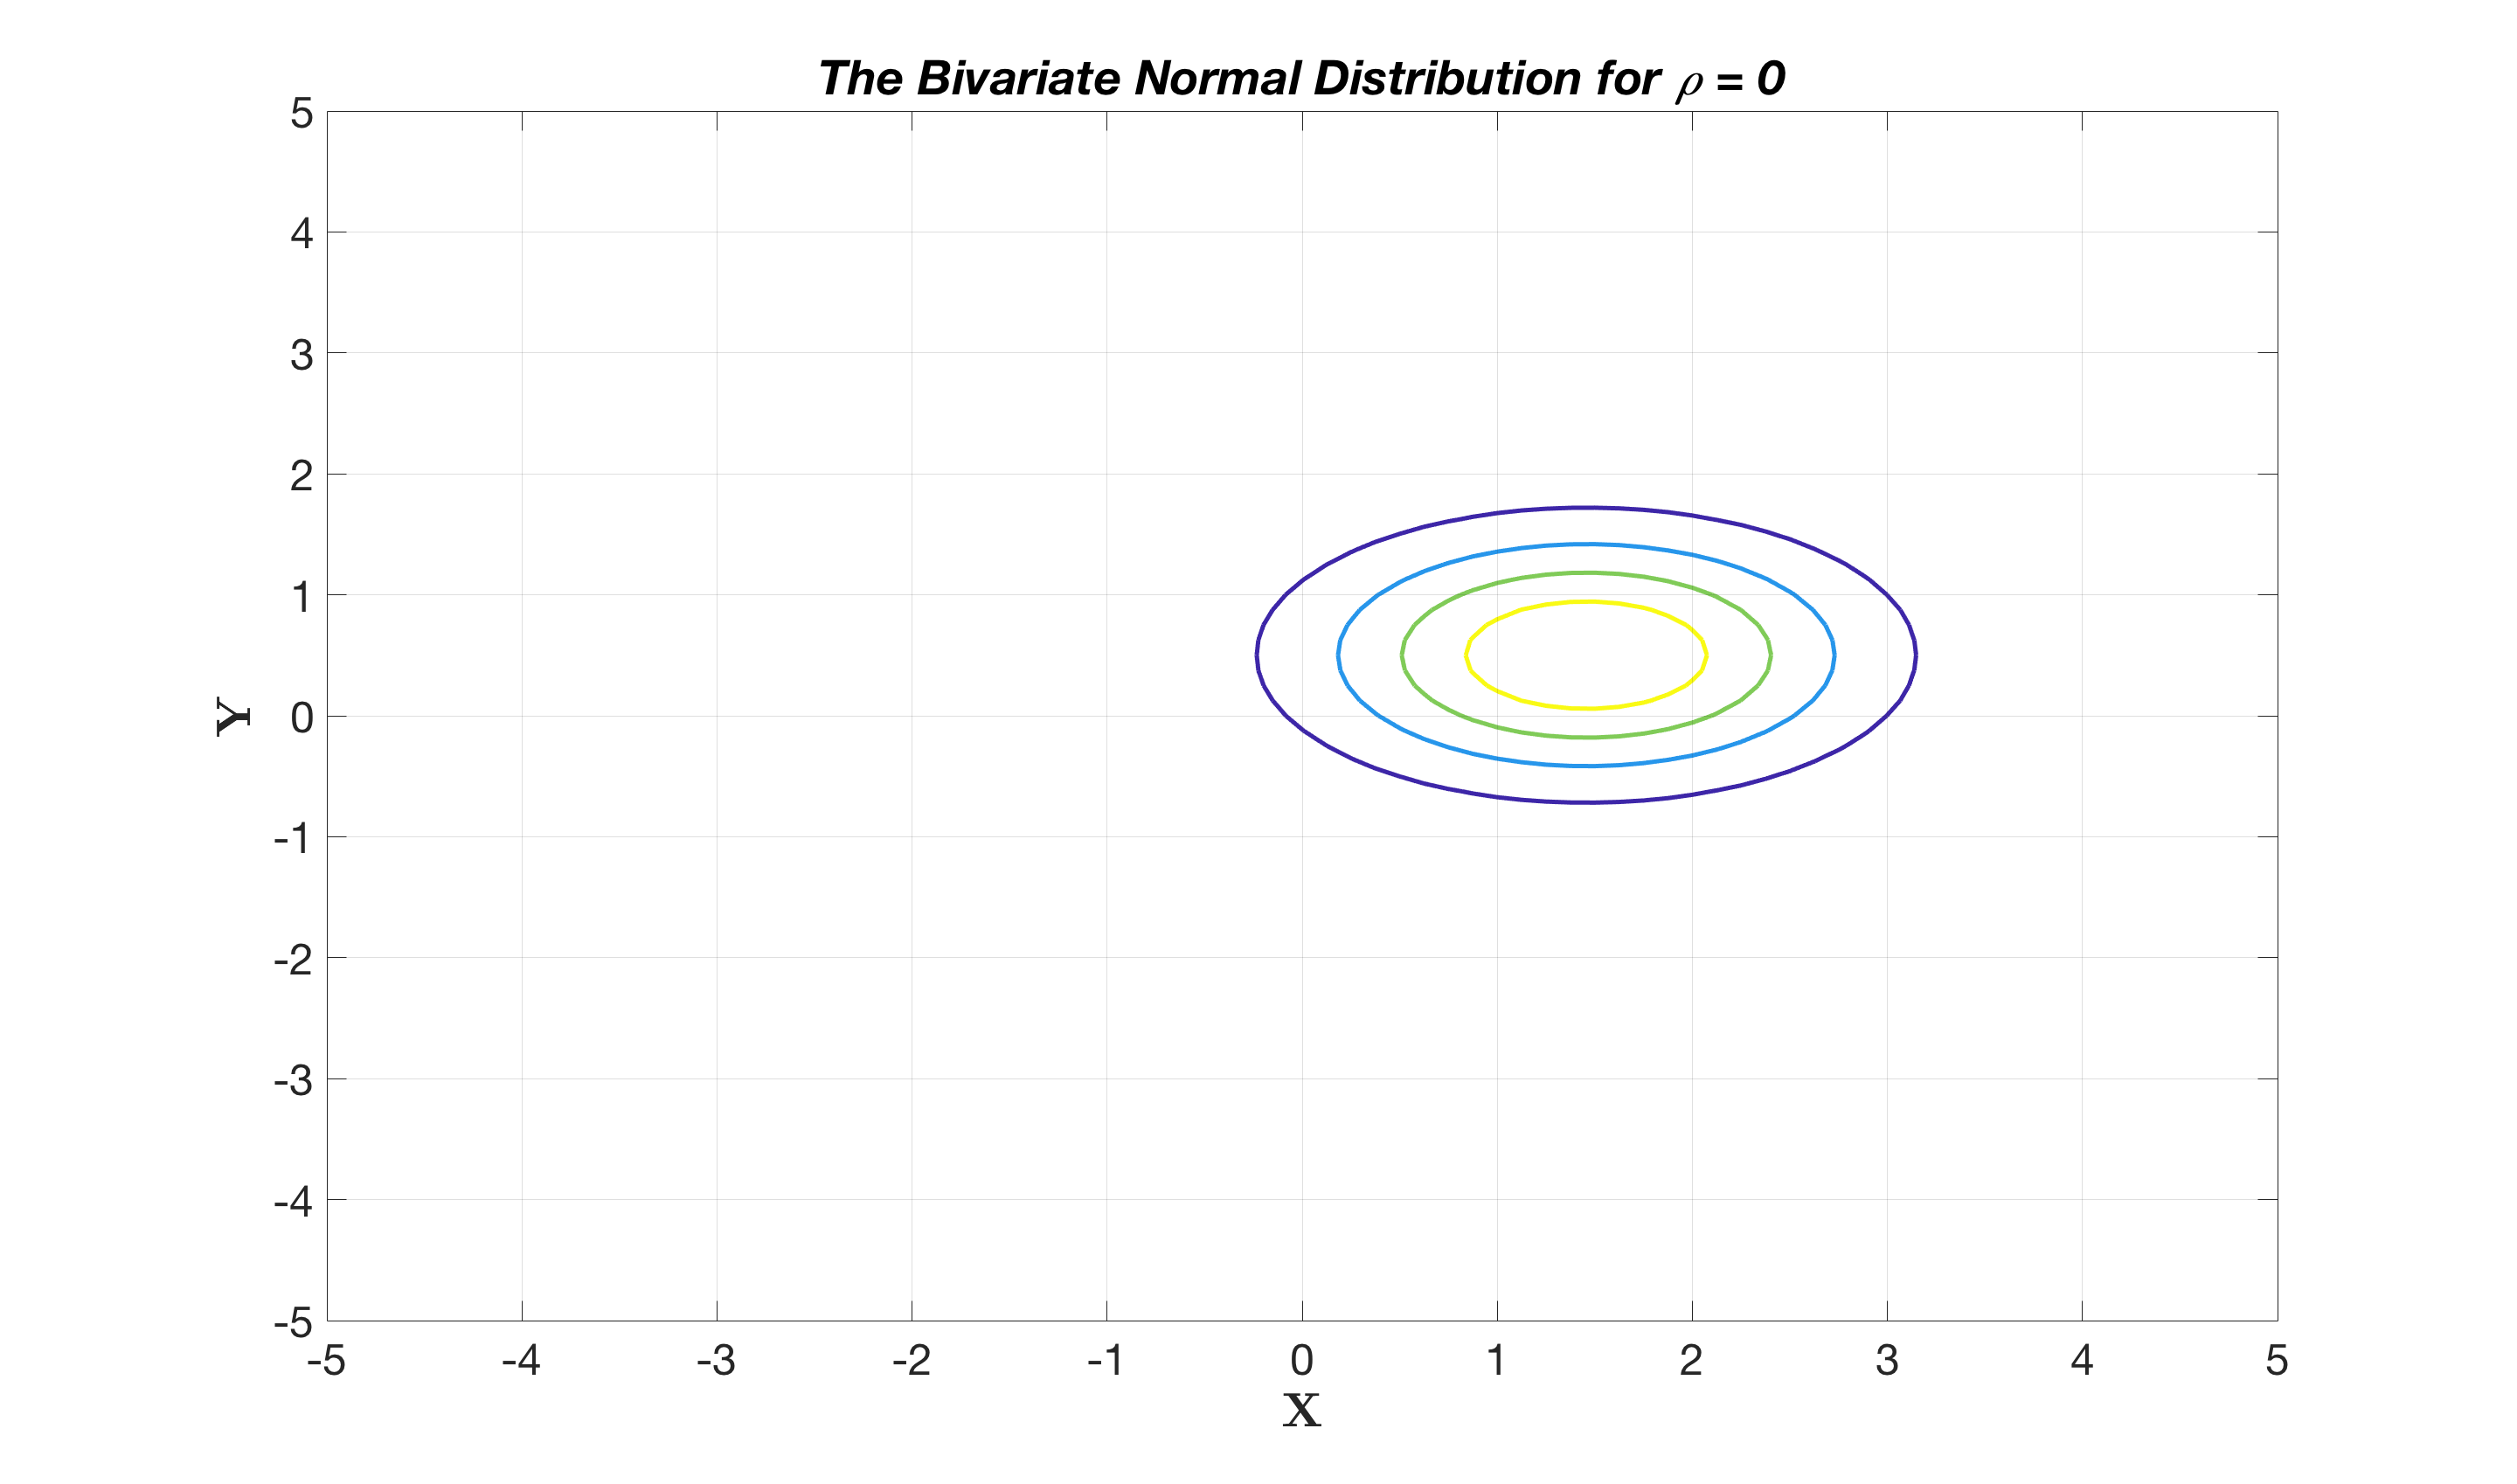
\includegraphics[width=.47\textwidth]{fig1.png}}\quad
   \subfloat[][]{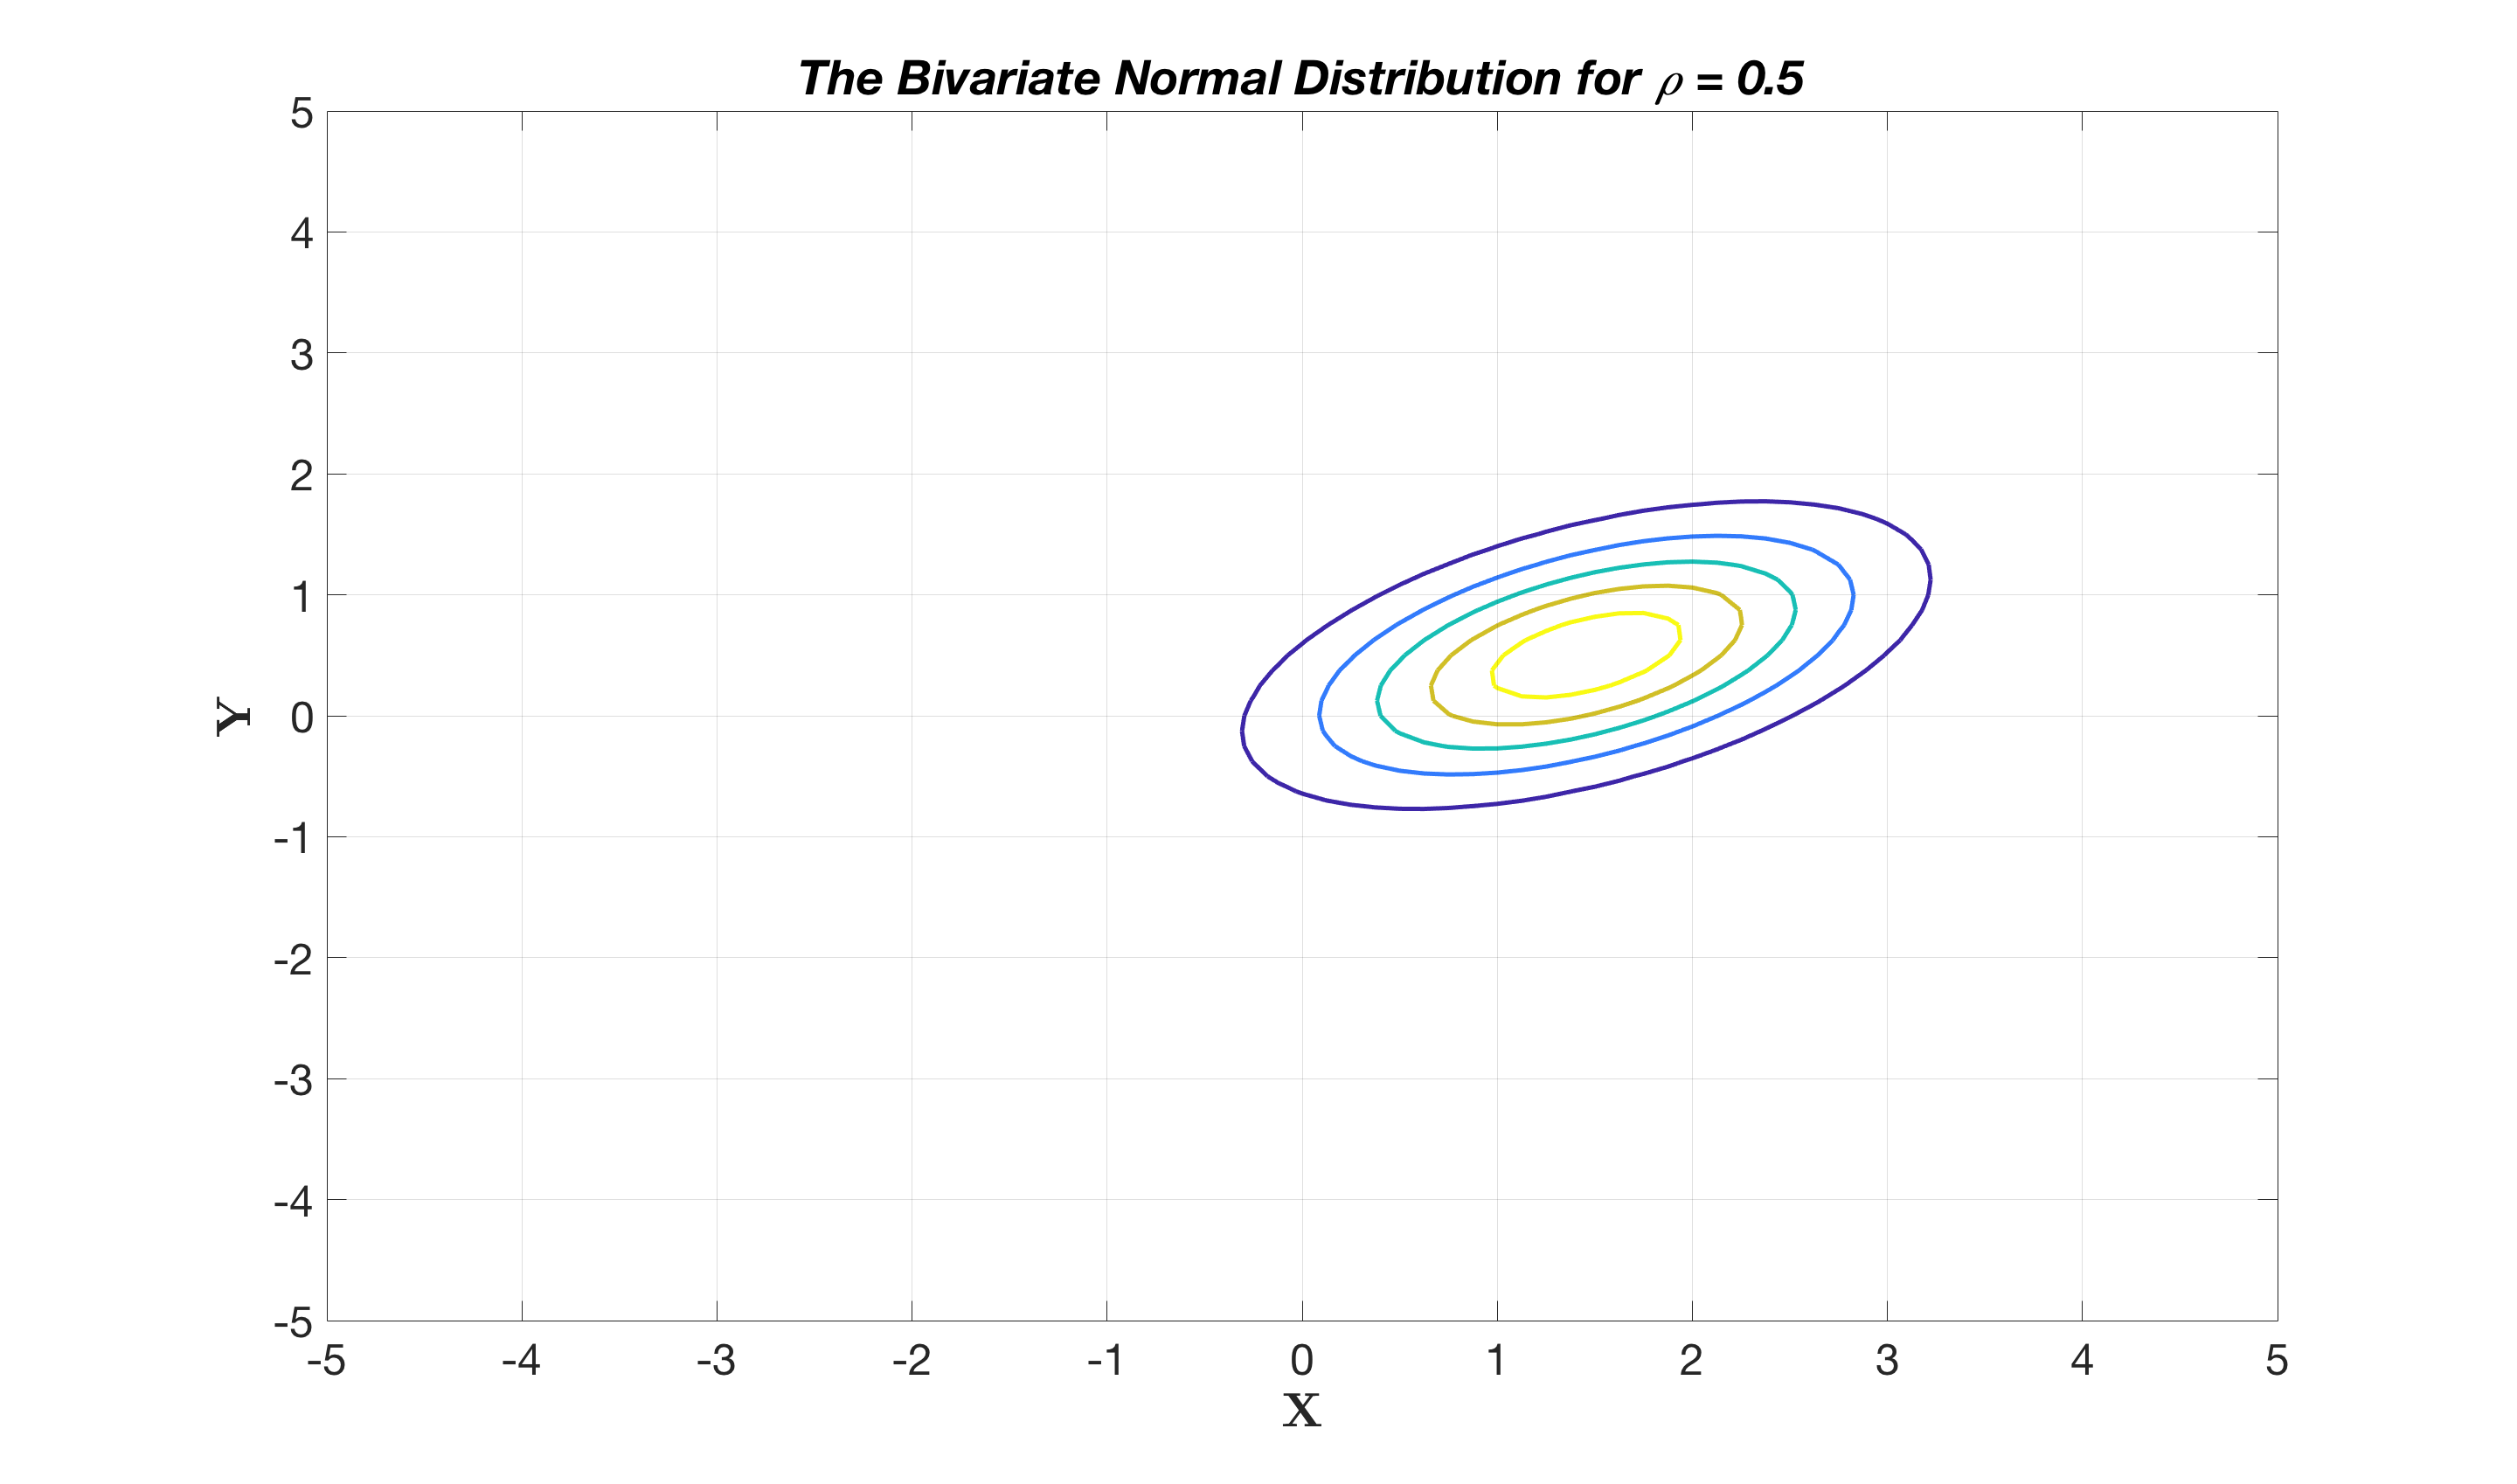
\includegraphics[width=.47\textwidth]{fig2.png}}\\
   \subfloat[][]{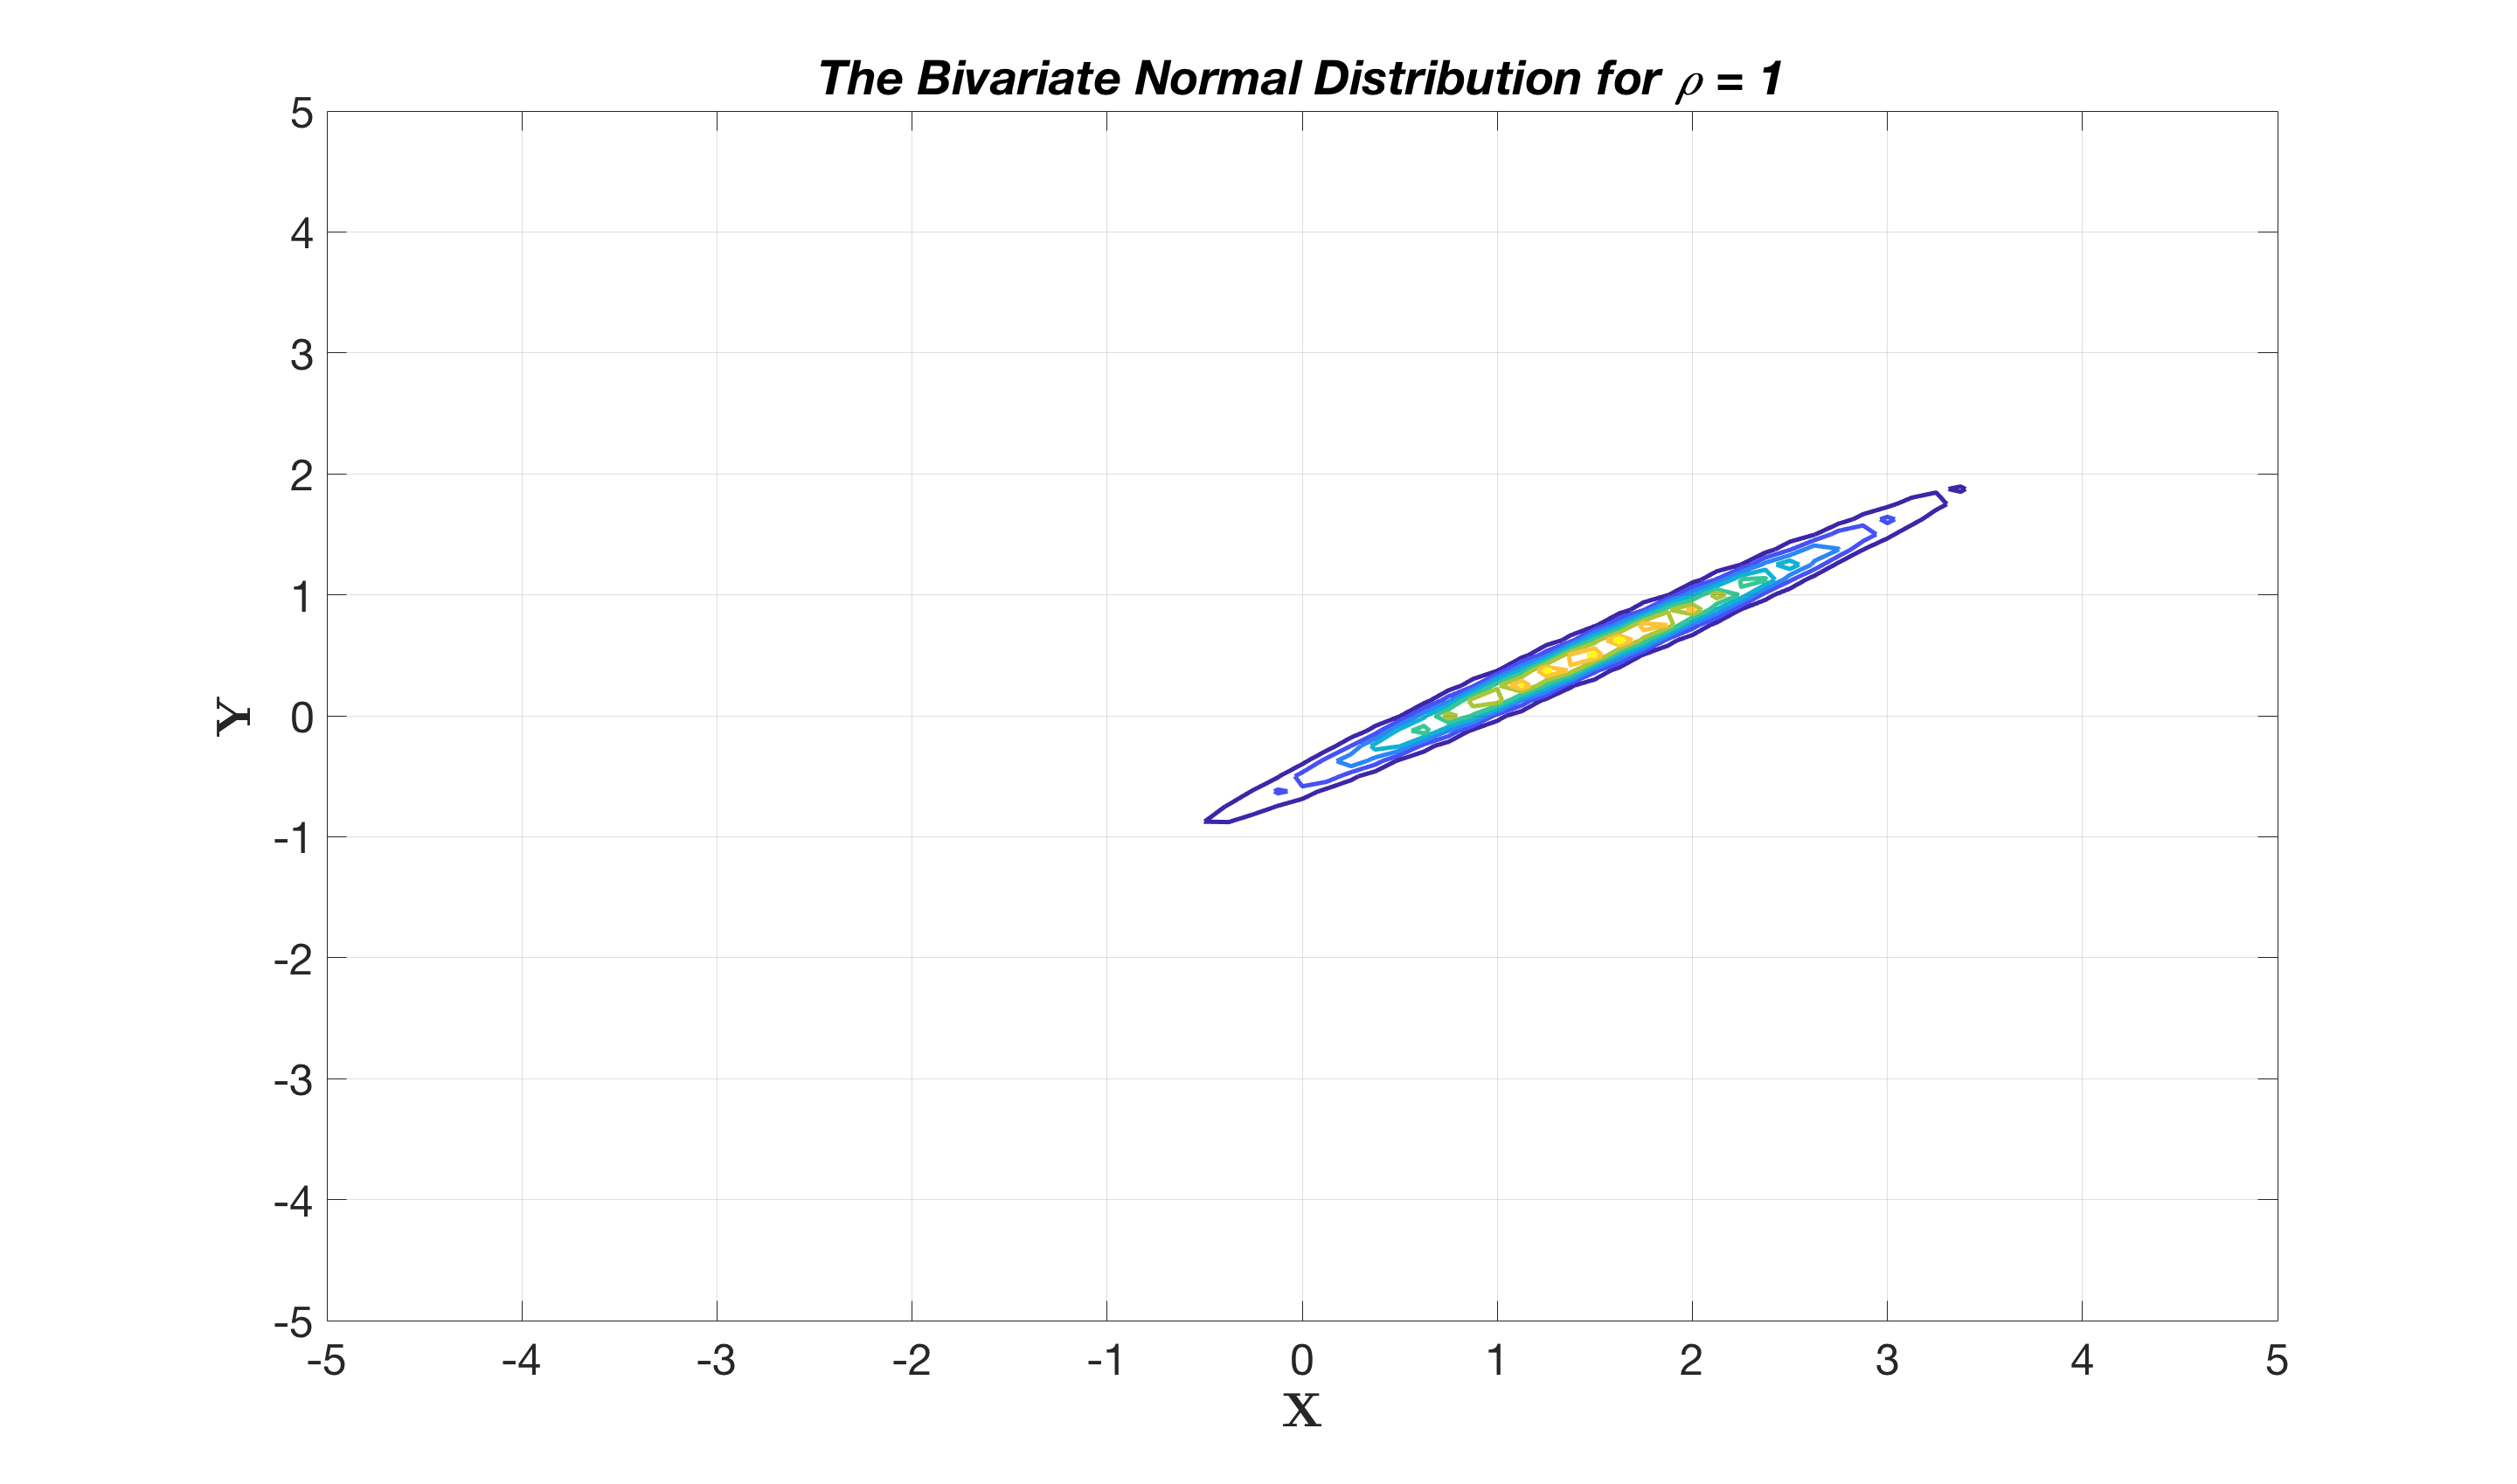
\includegraphics[width=.47\textwidth]{fig3.png}}\quad
   \subfloat[][]{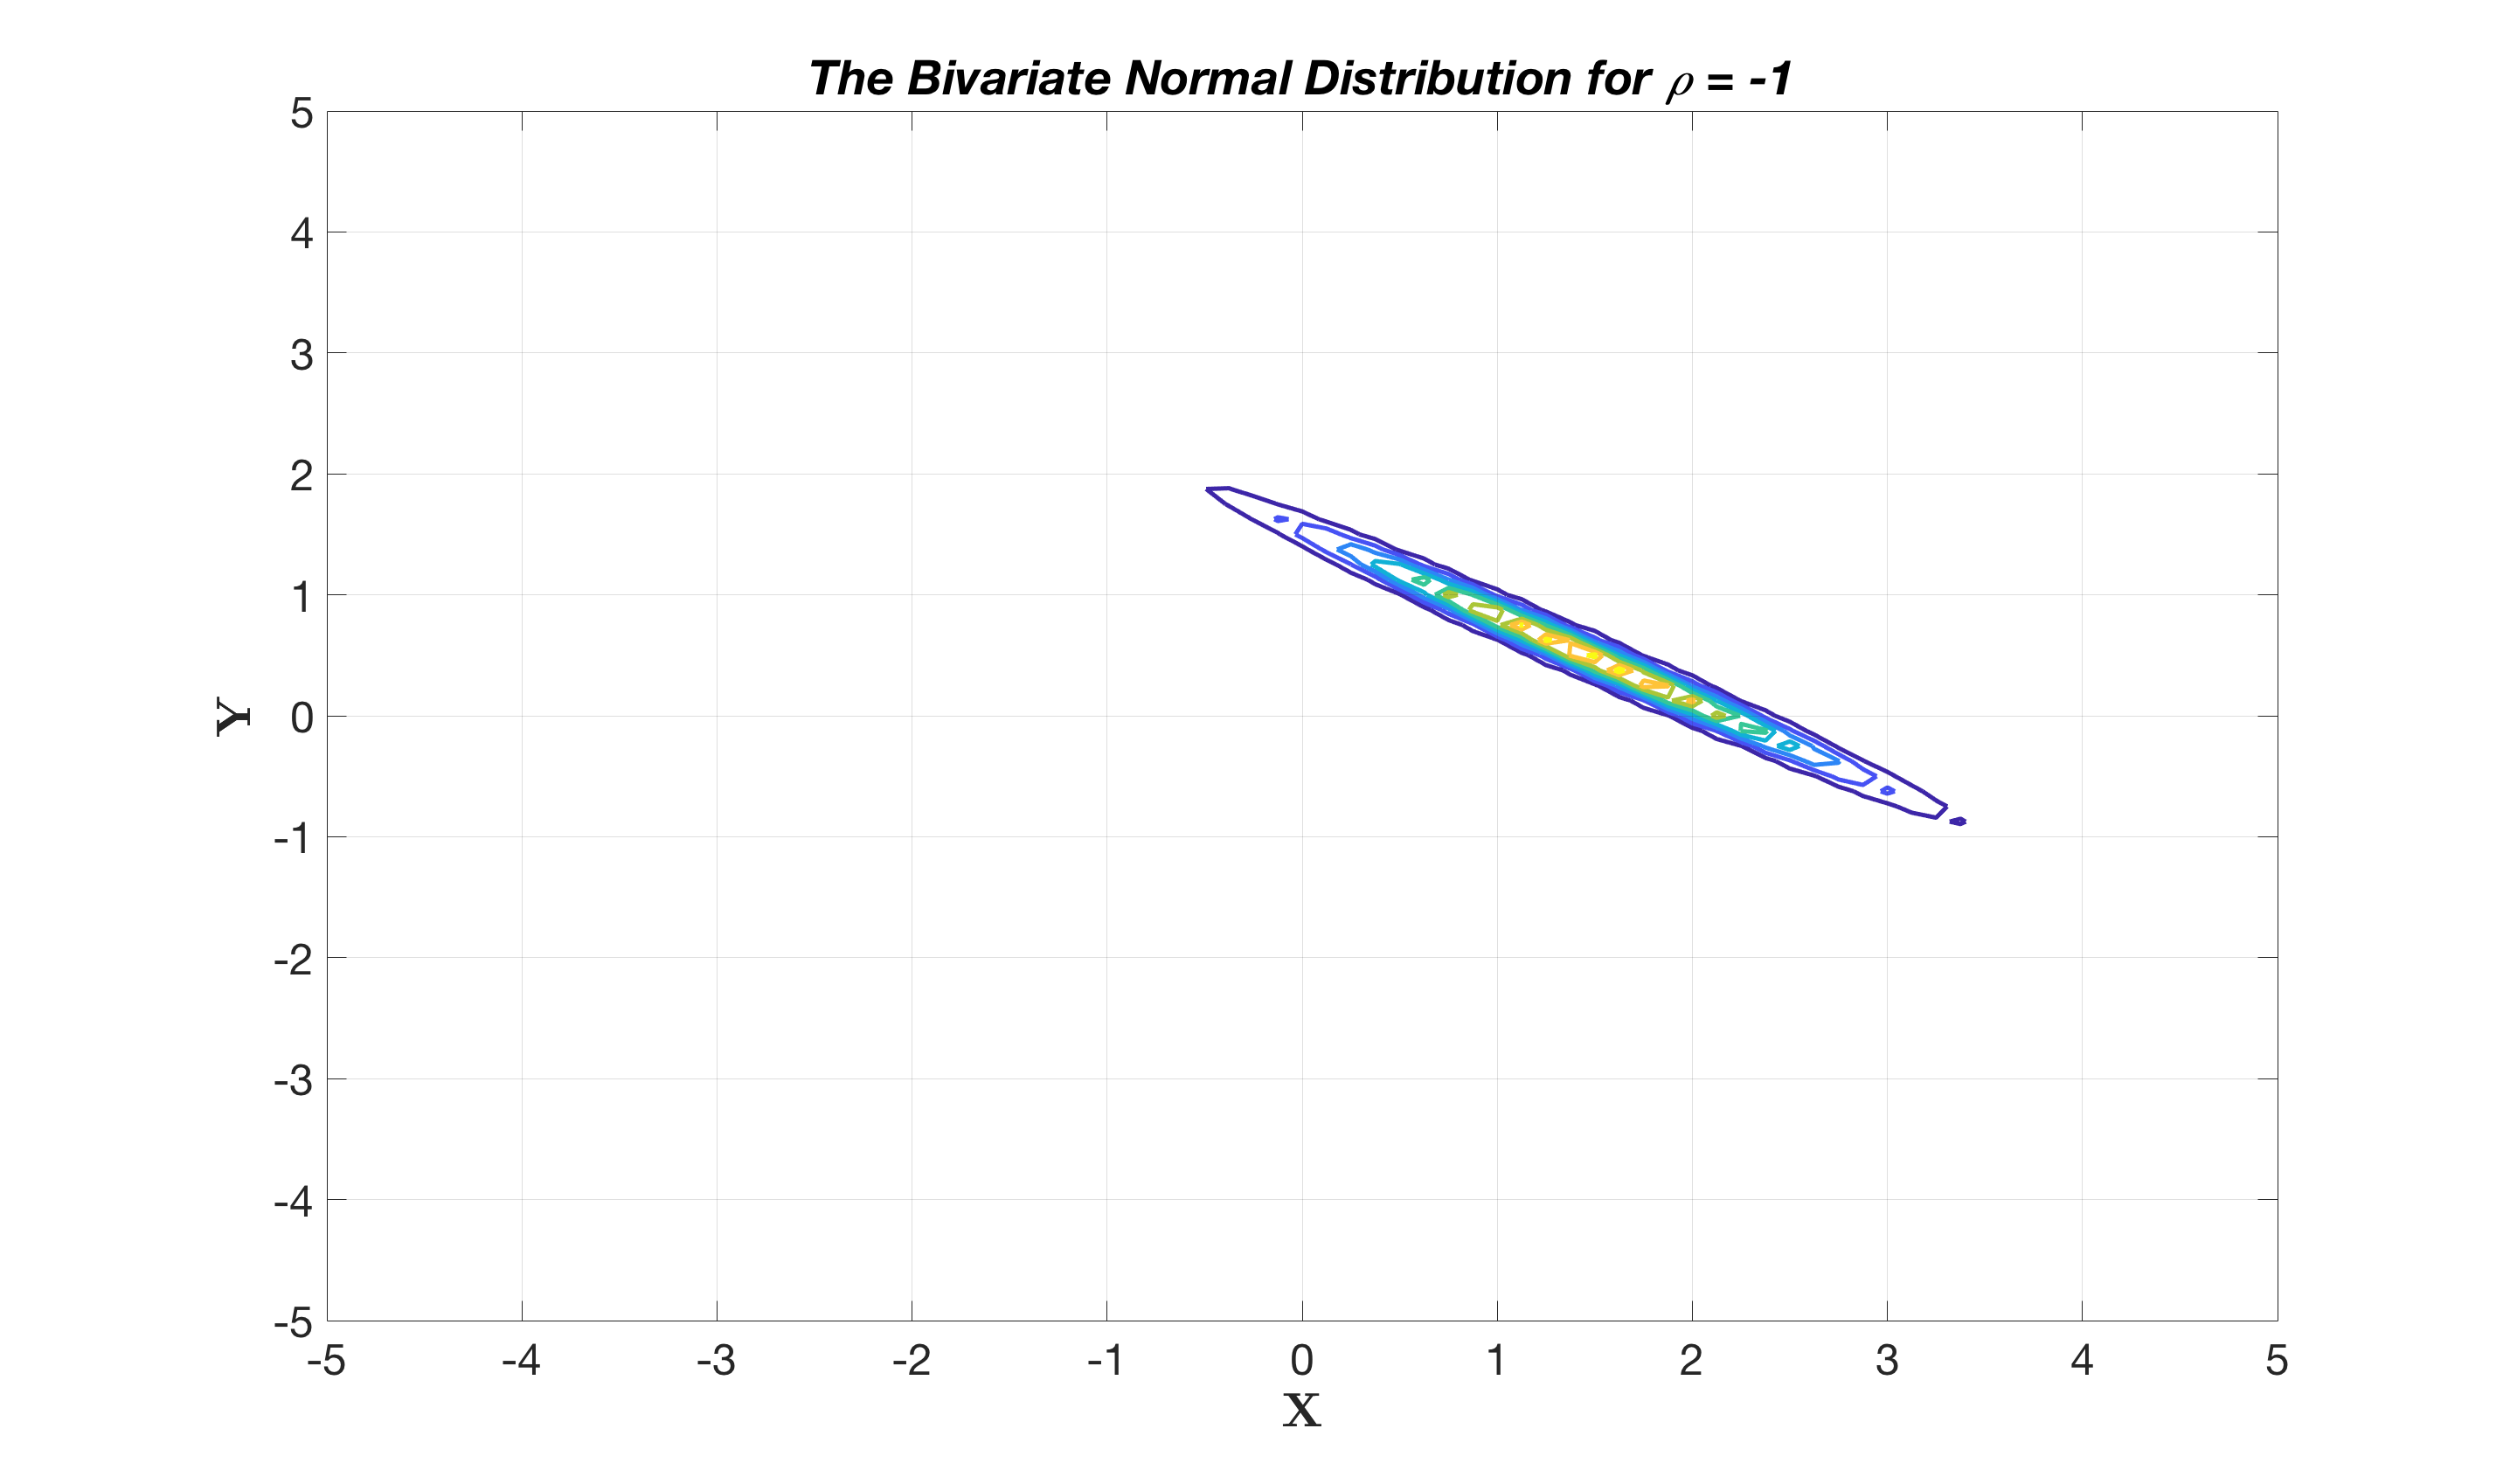
\includegraphics[width=.47\textwidth]{fig4.png}}
   \caption{Level curve for different values of $\rho$}
   \label{Level curve}
\end{figure}
\noindent The values of the parameters used in the density function is shown in the table. 

\begin{center}
 \begin{tabular}{*{4}{c}}
\toprule
$\mu_x$ & $\mu_y$ & $\sigma_x$  & $\sigma_x$ \\
\midrule
1.4569 & 0.5012 & 0.9435 & 0.6797 \\
\bottomrule
\hline
\end{tabular}
\end{center}

\noindent The first plot shows the case where the correlation $\rho$ is equal to zero. This special case is called the circular normal distribution. Here, we have a perfectly aligned ellipse. As $\rho$ increases, we can see that the curve becomes flattened in the perpendicular direction.

\section{Monte-Carlo-method}
\noindent \textbf{Task:} Develop a method for estimating the constant $\pi$ by using on the interval [0, 1] uniformly distributed random numbers. (Note: Consider pairs of these random numbers like coordinates of random points in the plane. How large is approximately the relative frequency that a point is lying inside the unit circle?) 

\noindent \textbf{Solution:} Monte Carlo simulation also known as MC simulation, is a method from Stochastics, in which a very large number of similar random experiments is the basis. It is an attempt made to numerically solve analytical problems that cannot be solved or only be solved with the help of probability theory. The constant $\pi$ can be estimated using Monte Carlo method as follows.
\begin{enumerate}
  \item We start shooting random points (x, y) within a unit square such that x, y belongs to [0 1]. The Figure 1.6 depicts a unit square along with a unit circle which is centred at (0, 0) and has radius 1.
   \begin{figure}[H]
    \centering
    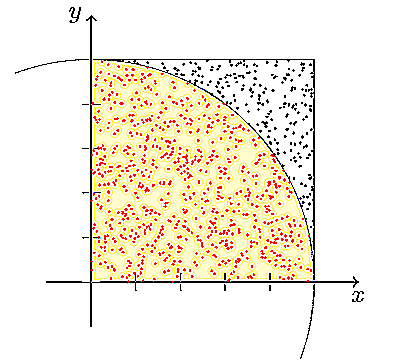
\includegraphics[width = .5\linewidth]{monte.png}
    \caption{Monte Carlo Method (example)}
  \end{figure}
 \item The random points (x, y) that lie inside that unit circle are coloured pink and those that lie on the unit square outside the circle are coloured black.
   \item We keep a track of the total number of points $N_{total}$ and the number of points inside the quarter unit circle $N_{circle}$
  \item If we divide $N_{circle}$ by $N_{total}$, we should get a value that is approximate to the ratio of area of the quarter circle to the area of the unit square. 
  $$\frac{N_{circle}}{N_{total}} =  \frac{\textit{Area of quarter circle}}{\textit{Area of unit square}}$$
$$\frac{N_{circle}}{N_{total}}= \frac{\frac{1}{4}\pi r^2}{r^2} = \frac{1}{4}\pi$$
\noindent Therefore,
$$\pi = 4*\frac{N_{circle}}{N_{total}}$$
 \item Thus $\pi$ can be estimated using the above equation. When we only have a small number of points, the estimation is not very accurate, but when we have hundreds of thousands of points, we get much closer to the actual value within around 2 decimal places of accuracy.
\end{enumerate}
\noindent It may take a long period to determine the value of $\pi$ using this experiment. As shown in the above figure, let the value of the radius of the circle be 1. We can calculate the distance from the origin using Pythagorean Theorem and the generated two random variables x and y. By knowing the value of the radius, the points hitting outside the circle can be easily differentiated from the points hitting within the circle. 

\noindent To estimate the value of $\pi$ in the interval [0,1] through the unit circle, two variables x and y has to be considered. Then the equilibrium can be given as, \\
$$\int_{0}^{1} \int_{0}^{\sqrt{1-x^2}}1 \textit{dy dx} \approx K/N $$
\noindent where, K = number of points within the circle, N = sample numbers